The infrastructure that currently serves the Drupal websites comprises 8 large physical Linux servers and a NAS shared filesystem.
It runs on CENTOS 7 and uses Puppet as configuration management system.
All servers run the same environment with Systemd services.
Major services are:
\begin{itemize}
    \item HAProxy load balancer: routes requests to worker nodes, with an affinity cookie
    \item Keepalived: implementation of floating IP for the load balancer
    \item Apache httpd: serves Drupal PHP code, WebDAV interface and a few additional PHP management applications
    \item php-fpm: maintains a pool of worker processes that generate Drupal content
\end{itemize}

\subsubsection*{Request journey}

When a request is made to a website on the infrastructure, eg home.cern, DNS resolves the name to the Drupal load balancer floating IP.
HAProxy then (hosted on 1 of the 8 servers) routes the request to one of the nodes.
Apache serves the request with Drupal PHP code. Drupal is configured to look up a directory for each site (multisite).
This flow can be seen in figure \ref{fig:drupal-physical-request-journey} together with the architecture.

Production websites respond to the load by spawning PHP workers, up to a maximum of 25.
A worker process is always listening for requests, even without load.
Test websites, on the other hand, spawn the first worker on demand and scale up to a maximum of 10 workers.
The PHP memory limit for every website is 512MB.

Websites have 2 data components: a directory and a database.
The directory lives on the NAS, shared among all servers.
The database is provided by an external dedicated service, Database on Demand (DBOD).

\begin{figure}[ht]
    \centering
    \hspace{-2em}
    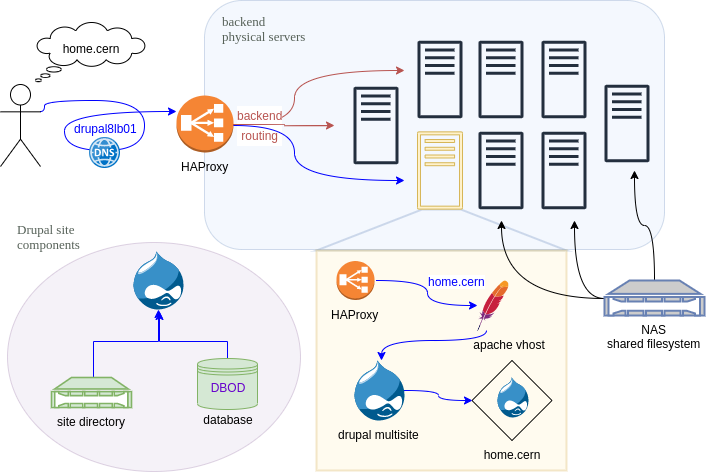
\includegraphics[width=\textwidth]{figures/drupal-physical-request-journey}
    \caption{\emph{Request journey in the physical infrastructure}.
    The current physical infrastructure consists of 8 physical Linux servers with a shared NAS filesystem.
    The {\color{blue} datapath} to access a site is shown in blue.
    The website's {\color{green} 2 data components}: a persistent directory on the NAS and a database on an external service (DBOD).
    }
    \label{fig:drupal-physical-request-journey}
\end{figure}

\subsubsection*{Website isolation}

Each website is assigned a Linux user.
Its directory is owned by it and not accessible by the users of other websites.
When Apache serves a request, it chroots the PHP process into the Drupal directory and sets the website's user.
This distinction provides a basic isolation mechanism.

Nevertheless, \emph{site isolation is relatively weak}.
We've never detected a cross-site security incident,
but there are no cgroup limits to resources, and not enough security layers to defend against privilege escalation exploits.
This is critical concern, given the vulnerability of CMS software \cite{shteiman_why_2014},
and the impact that defacing a high-traffic public site would have to CERN's reputation.

Furthermore, the website environment is inflexible.
All websites locked to the same Drupal version means massive, forced upgrade campaigns with little in the way of testing.
Better integration of testing and development environments is also lacking.

To top off the argument, the Drupal community is deprecating the multi-site functionality, % TODO ref
forcing us to adapt.

\subsection{Limitations of the current infrastructure}

Reiterating the discussion, these are the major limitations of the current infrastructure.
The Kubernetes infrastructure lifts all of them.

\begin{itemize}
    \item Hard to adjust resources, resulting in massive under-utilization
    \item Weak site isolation increases the risk of severe security incidents affecting multiple sites
    \item Inflexible website environment limits development \& testing workflows, makes upgrades cumbersome 
    \item \emph{Technical debt}: a lot of homebrew components built with legacy technologies specific to this system
\end{itemize}
